% !TeX spellcheck = de_DE
\documentclass{uebung_cs}
\usepackage{algo121}
\usepackage{algorithmic}
\blattname{Wochenplan: Stapel, Warteschlangen, Verkettete Listen und Bäume}

%%%%%%%%%%%%%%%%%%%%%%%%%%%%%%%%%%%%%%%%%%%%%%%%%%%%%%%%%%%%%%%%%%%%%%%%%%%%

\newboolean{programming}
\setboolean{programming}{true}

%%%%%%%%%%%%%%%%%%%%%%%%%%%%%%%%%%%%%%%%%%%%%%%%%%%%%%%%%%%%%%%%%%%%%%%%%%%%

\begin{document}

\section*{Vorbereitung}
Lies CLRS Einleitung von Teil III und Kapitel 10, Kapitel 17.4 bis Mitte von 17.4.1, und schau das Video der Woche.

\section*{Dienstag}

\begin{aufgabe}[Stapel und Warteschlangen]
	Löse die Teilaufgaben.
	\begin{enumerate}
		\item (\warmup) Betrachte einen anfangs leeren Stapel, auf dem die Operationen \texttt{PUSH(4)}, \texttt{PUSH(1)}, \texttt{PUSH(3)}, \texttt{POP()}, \texttt{PUSH(8)}, \texttt{POP()} ausgeführt werden. Wie sieht der Stapel nach jeder Operation aus, wenn dieser durch ein festes Feld der Länge 6 implementiert wurde?
		\item Wie können \emph{zwei} Stapel $S_1, S_2$ auf \emph{einem} festen Feld $A$ der Länge $N$ implementiert werden?
		Es darf hierbei zu keinem Überlauf kommen, es sei denn die Anzahl der Elemente in~$S_1$ und~$S_2$ ist größer als $N$.
		Die \texttt{PUSH} und \texttt{POP} Operationen sollen $O(1)$ Zeit benötigen.
		\item (\warmup) Betrachte eine anfangs leere Warteschlange, auf der die Operationen \texttt{ENQUEUE(4)}, \texttt{ENQUEUE(1)}, \texttt{ENQUEUE(3)}, \texttt{DEQUEUE()}, \texttt{ENQUEUE(8)}, \texttt{DEQUEUE()} ausgeführt werden. Wie sieht die Warteschlange nach jeder Operation aus, wenn diese auf einem festen Feld der Länge 6 implementiert wurde?
		\item (\hard) Wie können eine Warteschlange $Q$ und ihre Operationen durch zwei Stapel $S_1, S_2$ implementiert werden? (Zusätzliche Felder oder Objekte sind nicht erlaubt.)
		Analysiere die Laufzeit jeder Operation.
	\end{enumerate}
\end{aufgabe}

\begin{aufgabe}[Nahezu eine ehemalige dänische Klausuraufgabe]
	Sei $S$ ein Stapel.
	Führe die folgenden Operationen von links nach rechts aus: Ein Buchstabe $i$ steht hierbei für $S.$\texttt{PUSH(}$i$\texttt{)} und \verb|*| steht für $S.$\texttt{POP()}.
	\begin{verbatim}
		IFI*G**OE*THEU**NI
	\end{verbatim}
	Gib die Sequenz der Buchstaben an, die durch die \texttt{POP}-Aufrufe ausgegeben werden.
\end{aufgabe}

\begin{aufgabe}[Algorithmen auf verketteten Listen]
	Betrachte die Algorithmen \texttt{FOO} und \texttt{BAR} und die verkettete Liste darunter.
	\begin{center}
	\begin{minipage}{0.45\textwidth}
		\begin{algorithmic}
			\STATE \texttt{FOO}$(head)$
			\STATE $x = head$
			\STATE $c = 0$
			\WHILE{$x \neq null$}
				\STATE $x = x.next$
				\STATE $c = c + 1$
			\ENDWHILE
			\RETURN c
		\end{algorithmic}
	\end{minipage}%
		\hfill
	\begin{minipage}{0.45\textwidth}
		\begin{algorithmic}
			\STATE \texttt{BAR}$(x,s)$
			\IF{$x == null$}
				\RETURN s
			\ELSE
				\RETURN \texttt{Bar}$(x.next, s + x.key)$
			\ENDIF
		\end{algorithmic}
	\end{minipage}\\%
	\end{center}
	
	\begin{center}
		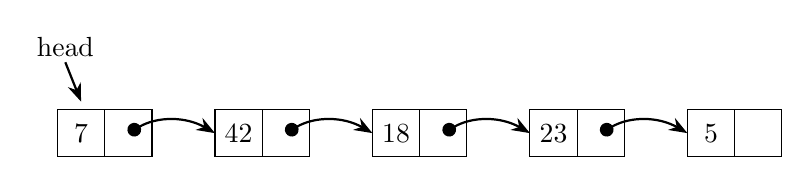
\begin{tikzpicture}
			\usetikzlibrary{arrows.meta}
			\def\list {7,42,18,23,5}  % list elements
			\def\listN {5} % number of elements in list
			\foreach \key [count=\index] in \list
			{
				% contours
				\draw (\index*2, 0.6) rectangle (\index*2 + 1.2, 0);
				\draw (\index*2+0.6,0.6) -- (\index*2+0.6,0);
				% key
				\node[] (k\index) at (\index*2+0.3, 0.3) {\key};
				% invisible nodes used for drawing pointers
				\node (left_of_\index) at (\index*2, 0.3) {};
				\node (next_\index) at (\index*2 + 0.9, 0.3) {};
			}
			\foreach \index in {2,...,\listN}
			{
				% pointer arrow
				\pgfmathtruncatemacro{\prev}{\index - 1};
				\draw[Circle-Stealth, thick, bend left=30] (next_\prev.center) to (left_of_\index.center);
			}
			% head pointer
			\node at (2.1,1.4) {head};
			\draw[-Stealth, thick] (2.1,1.2) to (2.3,0.7);
		\end{tikzpicture}	
	\end{center}

	\begin{enumerate}
		\item (\warmup) Führe \texttt{FOO}(head) händisch aus.
		\item (\warmup) Erkläre was \texttt{FOO} berechnet.
		\item Führe \texttt{BAR}(head, 0) händisch aus.
		\item Erkläre was \texttt{BAR} berechnet.
	\end{enumerate}
\end{aufgabe}

\begin{aufgabe}[Implementierung verketteter Listen, \warmup]
	Sei $x$ ein Element in einer einfach verketteten Liste wie in den Folien beschrieben.
	Löse die folgenden Teilaufgaben.
	\begin{enumerate}
		\item Sei $x$ nicht das letzte Element in der Liste.
		Worin resultiert der folgende Code-Schnipsel?
		\hspace*{20pt}\texttt{x.next = x.next.next;}

		\item Sei $t$ ein neues Element, das noch nicht in der Liste enthalten ist.
		Worin resultiert der folgende Code-Schnipsel?
		\hspace*{20pt}\texttt{t.next = x.next;}
		\hspace*{20pt}\texttt{x.next = t;}

		\item Voraussetzungen wie in b).
		Bringt der folgende Code-Schnipsel die gleichen Resultate?
		Wenn nein was sonst?
		\hspace*{20pt}\texttt{x.next = t;}
		\hspace*{20pt}\texttt{t.next = x.next;}
	\end{enumerate}
\end{aufgabe}

\ifthenelse{\boolean{programming}}{
\begin{aufgabe}[Implementierung von Stapeln und Warteschlangen]
	Implementiere die folgenden Datenstrukturen in einer Programmiersprache deiner Wahl.
	\begin{enumerate}
		\item Ein Stapel für Integer mittels einer einfach verketteten Liste.
		\item Eine Warteschlange für Integer mittels einer einfach verketteten Liste.
	\end{enumerate}
\end{aufgabe}
}{}

\section*{Donnerstag}

\begin{aufgabe}[Sortierte verkettete Listen]
	Sei $L$ eine einfach verkettete Liste von $n$ Integern in sortierter Reihenfolge.
	Löse die folgenden Aufgaben.
	\begin{enumerate}
		\item Entwirf einen Algorithmus, der einen neuen Integer in $L$ einfügt, sodass die Liste danach noch sortiert ist.
		\item Ein Freund schlägt vor, binäre Suche zu verwenden, um das Suchen in sortierten verketteten Listen zu beschleunigen. Wird das funktionieren? Begründe.
	\end{enumerate}
\end{aufgabe}

\begin{aufgabe}[Eine Liste umkehren]
	Entwirf einen Algorithmus, der eine einfach verkettete Liste $L$ mit $n$ Elementen als Eingabe erhält und diese umkehrt, das heißt, nach der Ausführung soll die Liste $L$ dieselben Elemente, jedoch in umgekehrter Reihenfolge enthalten.
	Der Algorithmus soll $O(n)$ Zeit brauchen und höchstens konstant viel zusätzlichen Speicherplatz benötigen.\footnote{Das heißt, der zusätzliche Speicherbedarf muss durch eine Konstante (unabhängig von $n$) beschränkt bleiben, selbst dann, wenn $n$ beliebig wächst.}
\end{aufgabe}

\begin{aufgabe}
	32 Inhaftierte sind zu lebenslänglicher Einzelhaft verurteilt.
	Der Gefängnisdirektor schlägt den Inhaftierten einen Deal vor, der zwar nicht mit Menschenrechten, jedoch mit einer algorithmischen Fragestellung vereinbar ist.
	Der Direktor hat eine Schüssel voller Zettel mit den Zellennummern aller Inhaftierten.
	Jeden Tag zieht der Direktor eine zufällige Nummer und lässt die inhaftierte Person aus der entsprechenden Zelle in das Vernehmungszimmer des Gefängnisses. Anschließend legt er die Zellennummer zurück in die Schüssel.
	Das Vernehmungszimmer ist leer, abgesehen von $k$ Lichtschaltern.
	Diese Lichtschalter können von den Inhaftierten an- und ausgeschaltet werden.
	Der Direktor schlägt folgenden Deal vor:
	Im Vernehmungszimmer angekommen, darf sich eine inhaftierte Person dazu entscheiden, laut zu sagen, dass alle 32 Inhaftierte mindestens einmal im Zimmer gewesen sein müssen.
	Liegt die Person mit ihrer Aussage richtig, werden alle Inhaftierten freigelassen.
	Liegt die Person mit ihrer Aussage falsch, werden alle Inhaftierten hingerichtet.
	Die Inhaftierten dürfen sich zu Beginn einmal treffen, um sich eine Strategie zu überlegen, bevor sie wieder voneinander isoliert werden.
	Anfangs sind alle Lichtschalter ausgeschaltet.
	
	\begin{enumerate}
		\item Ist es möglich für $k=32$ eine Strategie zu entwickeln, die mit 100\%iger Sicherheit funktioniert?
		\item Für $k=5$?
		\item (\veryhard) Für $k=1$?
	\end{enumerate}
\end{aufgabe}

\begin{aufgabe}[Dynamische Felder und Stapel]
	Wir wollen Stapel durch dynamische Felder implementieren.
	Löse die folgenden Teilaufgaben.
	\begin{enumerate}
		\item (\hard) Verallgemeinere die Implementierung durch dynamische Felder aus den Folien, sodass diese für Stapel sowohl \texttt{PUSH} als auch \texttt{POP} Operationen unterstützen.
		Wenn der Stapel anfangs leer ist und $n$ beliebige \texttt{PUSH}/\texttt{POP} Operationen ausgeführt werden, soll die Gesamtlaufzeit dieser $n$ Operationen $\Theta(n)$ betragen. Außerdem soll jede einzelne \texttt{PUSH} und \texttt{POP} Operation unabhängig vom Stapelinhalt maximale Laufzeit $O(n)$ haben.
		\item (\veryhard) Betrachte der Einfachheit halber nur die \texttt{PUSH} Operation.
		Zeige, wie man \texttt{PUSH} mithilfe dynamischer Felder so implementieren kann, dass die Laufzeit jeder einzelnen Operation $O(1)$ ist, also durch eine Konstante beschränkt.
		Hierbei soll der Speicherplatz linear in der Anzahl der auf dem Stapel enthaltenen Elemente sein.
		Wir nehmen für das Kostenmodell in dieser Aufgabe an, dass man ein Feld beliebiger Größe in Zeit $O(1)$ allokieren kann.\footnote{In C/C++ ist das einigermaßen realistisch, denn mit dem Codeschnipsel \texttt{int *array = malloc(n * sizeof(int))} sucht das Betriebssystem nach einem freien Speicherblock und allokiert diesen, ohne ihn zu durchlaufen. In Python stimmt das nicht, denn die ungefähr entsprechende Anweisung \texttt{array = [None for \_ in range(n)]} läuft in linearer Zeit ab. Wenn Sie Python gewohnt sind, dürfen Sie sich für diese Aufgabe also vorstellen, dass diese Python-Anweisung konstante Zeit bräuchte.}
		\textit{Hinweis:} Überlege, wie der Aufwand gleichmäßig über alle Operationen verteilt werden kann. 
	\end{enumerate}
\end{aufgabe}

\end{document}
